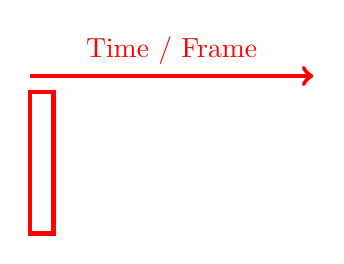
\begin{tikzpicture}
    \def\boxwidth{0.3}

    \coordinate (Row1) at (0,0);
    \coordinate (Row2) at (0,\boxwidth);
    \coordinate (Row3) at (0,2*\boxwidth);
    \coordinate (Row4) at (0,3*\boxwidth);
    \coordinate (Row5) at (0,4*\boxwidth);
    %\coordinate (Row5) at (0,5*\boxwidth);

    % Layer 1

    %\draw[color=red, ultra thick] (0,0) rectangle (12*\boxwidth, 6*\boxwidth);

    \draw[color=red, ultra thick] (0,0) rectangle (\boxwidth, 6*\boxwidth);

    \draw[color=red, ->, ultra thick] (0, 6*\boxwidth+0.2) -- (12*\boxwidth, 6*\boxwidth+0.2) node [anchor=south, midway] {Time / Frame};

\end{tikzpicture}